\begin{quote}
A systematic presentation removes ideas from the ground that made them
grow and arranges them in an artificial pattern.

--- Paul Feyerabend, \emph{The Tyranny of Science}, Polity Press (2011)
\end{quote}

\begin{quote}
Irony is said to allow the artist to continue his creative production
while immersed in a sociocultural context of which he is critical.

--- Emmanuel Petit, \emph{Irony or, the Self-Critical Opacity of
Postmodernist Architecture}, Yale (2013)
\end{quote}

\hypertarget{introduction}{%
\section{Introduction}\label{introduction}}

Many forms of software have been developed to enable programming. The
classic form consists of a \emph{programming language}, a text editor to
enter source code, and a compiler to turn it into an executable program.
Instances of this form are differentiated by the syntax and semantics of
the language, along with the implementation techniques in the compiler
or runtime environment. Since the advent of graphical user interfaces
(GUIs), programming languages can be found embedded within graphical
environments that increasingly define how programmers work with the
language---for instance, by directly supporting debugging or
refactoring. Beyond this, the rise of GUIs also permits diverse visual
forms of programming, including visual languages and GUI-based end-user
programming tools. This paper advocates a shift of attention from
\emph{programming languages} to the more general notion of ``software
that enables programming''---in other words, \emph{programming systems}.

A \emph{programming system} may include tools, protocols, notations,
interfaces, and languages. It is a software artifact that makes it
possible to construct programs, debug them, and turn them into
operational, maintained, and evolvable artifacts running on appropriate
hardware. This notion covers classic programming languages together with
their editors, debuggers, compilers, and other tools. Yet it is
intentionally broad enough to accommodate image-based programming
environments like Smalltalk, operating systems like UNIX, and hypermedia
authoring systems like Hypercard, in addition to various other examples
we will mention.

\hypertarget{what-is-the-problem}{%
\subsection{What is the problem?}\label{what-is-the-problem}}

There is a growing interest in broader forms of \emph{programming
systems}, both in the programming research community and in industry. On
the one hand, researchers are studying topics such as \emph{programming
experience} and \emph{live programming} that require considering not
just the \emph{language}, but further aspects of a given system. On the
other hand, commercial companies are building new programming
environments like Replit \cite{ReplitWeb} or low-code tools like Dark
\cite{DarkWeb} and Glide \cite{GlideWeb}. Yet, such topics remain at the
sidelines of mainstream programming research. While \emph{programming
languages} are a well-established concept, analysed and compared in a
common vocabulary, no similar foundation exists for the wider range of
\emph{programming systems}.

The academic research on programming suffers from this lack of common
vocabulary. While we may thoroughly assess programming \emph{languages},
as soon as we add interaction or graphics into the picture, we often get
stuck on how the resulting system is vaguely ``interesting''. Moreover,
when designing new systems, inspiration is often drawn from the same few
standalone sources of ideas. These might be influential past systems
like Smalltalk, programmable end-user applications like spreadsheets, or
motivational illustrations by thinkers like Victor~\cite{BretVictor}.

Instead of forming a solid body of work, the ideas that emerge are
difficult to relate to each other. The research methods used to study
programming systems lack the rigorous structure of programming language
research methods. They tend to rely on singleton examples, which
demonstrate the author's ideas, but are inadequate methods for comparing
new ideas with the work of others. This makes it hard to build on top
and thereby advance the state of the art.

Studying \emph{programming systems} is not merely about taking a
programming language and looking at the tools that surround it. It
presents a \emph{paradigm shift} to a perspective that is, at least
partly, \emph{incommensurable} with that of languages. When studying
programming languages, everything that matters is in the program code;
when studying programming systems, everything that matters is in the
\emph{interaction} between the programmer and the system. As documented
by Gabriel \cite{PLrev}, looking at a \emph{system} from a
\emph{language} perspective makes it impossible to think about concepts
that arise from interaction with a system, but are not reflected in the
language. Thus, we must proceed with some caution. As we will see, when
we talk about Lisp as a programming system, we mean something very
different from a parenthesis-heavy programming language!

\hypertarget{contributions}{%
\subsection{Contributions}\label{contributions}}

We propose a common language as an initial step towards a more
progressive research on programming systems. Our set of \emph{technical
dimensions} seeks to break down the holistic view of systems along
various specific ``axes''. The dimensions identify a range of possible
design choices, characterized by two extreme points in the design space.
They are not quantitative, but they allow comparison by locating systems
on a common axis. We do not intend for the extreme points to represent
``good'' or ``bad'' designs; we expect any position to be a result of
design trade-offs. At this stage we encourage agreement on descriptions
of systems first, in order to settle any normative judgements later.

The set of dimensions can be understood as a map of the design space of
programming systems (Figure~\ref{fig:tech-dims-diagram}). Past and
present systems will serve as landmarks, and with enough of them,
unexplored or overlooked possibilities will reveal themselves. So far,
the field has not been able to establish a virtuous cycle of feedback;
it is hard for practitioners to situate their work in the context of
others' so that subsequent work can improve on it. Our aim is to provide
foundations for the study of programming systems that would allow such
development.

This paper is intended as a reference on the current state of the
technical dimensions framework and it is meant to be \emph{used} rather
than \emph{read}. We present the dimensions in detail, but encourage the
reader to skim through the details on the first read. Subsequently, we
suggest revisiting dimensions which seem relevant to a concrete system
known to the reader. The main contributions of this paper are organized
as follows:

\begin{enumerate}
\def\labelenumi{\arabic{enumi}.}
\tightlist
\item
  In Section~\ref{programming-systems}, we characterize what a
  programming system is and review landmark programming systems of the
  past that are used as examples throughout this paper, as well as to
  delineate our notion of a programming system.
\item
  In Section~\ref{technical-dimensions}, we present the technical
  dimensions in details, organised into related clusters:
  \emph{interaction}, \emph{notation}, \emph{conceptual structure},
  \emph{customizability}, \emph{complexity}, \emph{errors}, and
  \emph{adoptability}. For each technical dimension, we give examples
  that illustrate a number of values along the axis identified by the
  dimension.
\item
  In Section~\ref{discussion}, we sketch two ways of using the technical
  dimensions framework. In Section~\ref{evaluating-programming-systems},
  we use it to evaluate a recent interesting programming system and in
  Section~\ref{exploring-the-design-space}, we use it to identify an
  unexplored point in the design space and envision a potential novel
  programming system.
\end{enumerate}

\begin{figure}
  \centering
  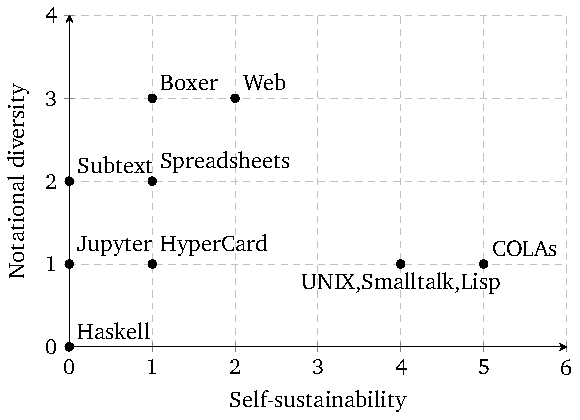
\includegraphics[width=0.6\linewidth]{plot-figure0.pdf}
  \caption{One 2-dimensional slice of the space of possible systems, to be examined in more detail in Section\ \ref{exploring-the-design-space}.\label{fig:tech-dims-diagram}}
\end{figure}

\hypertarget{related-work}{%
\section{Related work}\label{related-work}}

While we do have new ideas to propose, part of our contribution is
integrating a wide range of \emph{existing} concepts under a common
umbrella. This work is spread out across different domains, but each
part connects to programming systems or focuses on a specific
characteristic they may have.

\paragraph{From languages to systems.}

Our approach lies between a narrow focus on programming languages and a
broad focus on programming as a socio-political and cultural subject.
Our concept of a programming system is technical in scope, although we
acknowledge the technical side often has important social implications
as in the case of the ``Adoptability'' dimension
(Section~\ref{adoptability}). This contrasts with the more
socio-political focus found in Tchernavskij \cite{TcherDiss} or in
software studies \cite{SwStudies}. It overlaps with Kell's
conceptualization of UNIX, Smalltalk, and Operating Systems
generally~\cite{KellOS}, and we have ensured that UNIX has a place in
our framework.

The distinction between more narrow \emph{programming languages} and
broader \emph{programming systems} is more subtle. Richard Gabriel noted
an invisible paradigm shift from the study of ``systems'' to the study
of ``languages'' in computer science \cite{PLrev}, and this observation
informs our distinction here. One consequence of the change is that a
\emph{language} is often formally specified apart from any specific
implementations, while \emph{systems} resist formal specification and
are often \emph{defined by} an implementation. We recognize programming
language implementations as a \emph{small region} of the space of
possible systems (Figure~\ref{fig:tech-dims-diagram}). Hence we refer to
the \emph{interactive programming system} aspects of languages, such as
text editing and command-line workflow.

\paragraph{Programming systems research.}

There is renewed interest in programming systems in both industry and
research, but the holistic programming systems view is more often
adopted in work on non-traditional programming tools:

\begin{itemize}
\tightlist
\item
  Computational notebooks such as Jupyter simplify data analysis by
  combining code snippets with text and visual output. They are backed
  by stateful ``kernels'' and used interactively.
\item
  ``Low code'' end-user programming systems allow application
  development (mostly) through a GUI. One example is Coda
  \cite{CodaWeb}, which combines tables, formulas, and scripts to enable
  non-technical people to build ``applications as documents''.
\item
  Domain-specific programming systems such as Dark, which claims a
  ``holistic'' programming experience for cloud API services. This
  includes a language, a direct manipulation editor, and
  near-instantaneous building and deployment.
\item
  Even for general purpose programming with conventional tools, systems
  like Replit have demonstrated the benefits of integrating all needed
  languages, tools, and user interfaces into a seamless experience,
  available from the browser, that requires no setup.
\end{itemize}

Research that follows the programming systems perspective can be found
in a number of research venues. Those include Human-Computer Interaction
conferences such as \href{https://uist.acm.org/}{UIST}\footnote{ACM
  Symposium on User Interface Software and Technology} and
\href{https://conferences.computer.org/VLHCC/}{VL/HCC}\footnote{IEEE
  Symposium on Visual Languages and Human-Centric Computing}. However,
work in those often emphasizes the user experience over technical
description. Programming systems are often presented in workshops such
as \href{https://liveprog.org/}{LIVE} and
\href{https://2021.programming-conference.org/home/px-2021}{PX}\footnote{Programming
  eXperience}. However, work in those venues is often limited to the
authors' individual perspectives and suffers from the aforementioned
difficulty of comparing to other systems.

Concrete examples of systems appear throughout the paper. Recent systems
which motivated some of our dimensions include Subtext \cite{Subtext},
which combines code with its live execution in a single editable
representation; Sketch-n-sketch \cite{SnS}, which can synthesize code by
direct manipulation of its outputs; Hazel \cite{Hazel}, a live
functional programming environment with typed holes to enable execution
of incomplete or ill-typed programs; and Webstrates \cite{Webstrates},
which extends Web pages with real-time sharing of state.

\paragraph{Already-known characteristics.}

There are several existing projects identifying characteristics of
programming systems. Some revolve around a single one, such as levels of
liveness \cite{Liveness}, or plurality and communicativity
\cite{KellComm}. Others propose an entire collection. \emph{Memory
Models of Programming Languages}~\cite{MemMod} identifies the
``everything is an X'' metaphors underlying many programming languages;
the \emph{Design Principles of Smalltalk}~\cite{STdesign} documents the
philosophical goals and dicta used in the design of Smalltalk; the
``Gang of Four'' \emph{Design Patterns}~\cite{DesPats} catalogues
specific implementation tactics; and the \emph{Cognitive Dimensions of
Notation}~\cite{CogDims} introduces a common vocabulary for software's
\emph{notational surface} and for identifying their trade-offs.

The latter two directly influence our proposal. Firstly, the Cognitive
Dimensions are a set of qualitative properties which can be used to
analyze \emph{notations}. We wish to extend this approach to the
``rest'' of a system, beyond its notation, with \emph{Technical}
Dimensions. Secondly, our individual dimensions naturally fall under
larger \emph{clusters} that we present in a regular format, similar to
the presentation of the classic Design Patterns. As for characteristics
identified by others, part of our contribution is to integrate them
under a common umbrella: liveness, pluralism, and uniformity metaphors
(``everything is an X''), which have already been identified by others,
become dimensions in our framework.

\paragraph{Methodology.}

We follow the attitude of \emph{Evaluating Programming
Systems}~\cite{EvProgSys} in distinguishing our work from HCI methods
and empirical evaluation. We are generally concerned with
characteristics that are not obviously amenable to statistical analysis
(e.g.~mining software repositories) or experimental methods like
controlled user studies, so numerical quantities are generally not
featured.

Similar development seems to be taking place in HCI research focused on
user interfaces. The UIST guidelines \cite{UISTAuthor} instruct authors
to evaluate system contributions holistically, and the community has
developed heuristics for such evaluation, such as \emph{Evaluating User
Interface Systems Research}~\cite{EvUISR}. Our set of dimensions offers
similar heuristics for identifying interesting aspects of programming
systems, though they focus more on underlying technical properties than
the surface interface.

Finally, we believe that the aforementioned paradigm shift from
programming systems to programming languages has hidden many ideas about
programming that are worthwhile recovering and developing further
\cite{ComplementaryBasic}. Thus our approach is related to the idea of
\emph{complementary science} developed by Chang~\cite{Chang} in the
context of history and philosophy of science. Chang argues that even in
disciplines like physics, superseded or falsified theories may still
contain interesting ideas worth documenting. In the field of
programming, where past systems are discarded for many reasons besides
empirical failure, Chang's \emph{complementary science} approach seems
particularly suitable.

\paragraph{Programming systems deserve a theory too!}

In short, while there is a theory for programming languages, programming
\emph{systems} deserve a theory too. It should apply from the small
scale of language implementations to the vast scale of operating
systems. It should be possible to analyse the common and unique features
of different systems, to reveal new possibilities, and to build on past
work in an effective manner. In Kuhnian terms, it should enable a body
of ``normal science'': filling in the map of the space of possible
systems (Figure \ref{fig:tech-dims-diagram}), thereby forming a
knowledge repository for future designers.

\hypertarget{programming-systems}{%
\section{Programming systems}\label{programming-systems}}

We introduce the notion of a \emph{programming system} through a number
of examples, classified following the style of Lehman \cite{SPEPrograms}
into three broad types. These are loosely inspired by the notions of
\emph{languages}, \emph{operating systems} and \emph{applications}:

\begin{itemize}
\item
  \textbf{L-type programming systems} are software ecosystems built
  around a text-based programming \emph{language}. They consist of a set
  of tools such as compilers, debuggers, and profilers. These tools may
  exist as separate command-line programs, or within an Integrated
  Development Environment.
\item
  \textbf{O-type programming systems} resemble \emph{operating systems}
  in that they structure the execution environment and encompass the
  resources of an entire machine (physical or virtual). They provide a
  common interface for communication, both between the user and the
  computer, and between programs themselves.
\item
  \textbf{A-type programming systems} are programmable
  \emph{applications}. They are typically optimized for a specific
  domain, and offer a limited degree of programmability which may be
  increased with newer versions.
\end{itemize}

We will illustrate each of these types with several examples. This will
provide an intuition for the notion of a programming system and
establish a collection of go-to examples for the rest of the paper.

\hypertarget{l-type-programming-systems}{%
\subsection{L-type programming
systems}\label{l-type-programming-systems}}

We see programming systems as (collections of) software artifacts that
make it possible to construct programs, debug them, and turn them into
operational, maintained, and evolvable artifacts running on an
appropriate hardware. Text-based programming languages sit within
programming systems whose boundaries are not explicitly defined. To
speak of a programming system, we need to consider a language with, at
minimum, an editor and a compiler or interpreter. However, the exact
boundaries are a design choice that significantly affects our analysis.

\paragraph{Java with the Eclipse ecosystem.}

Java cannot be viewed as a programming system on its own, but it is one
if we consider it as embedded in an ecosystem of tools. There are
multiple ways to delineate this, resulting in different analyses. A
minimalistic programming system would consist of a text editor to write
Java code and a command line compiler. A more realistic system is Java
as embedded in the Eclipse IDE. The programming systems view allows us
to see all there is beyond the textual code. In the case of Eclipse,
this includes the debugger, refactoring tools, testing and modelling
tools, GUI designers, and so on. This delineation yields a programming
system that is powerful and convenient, but has a large number of
concepts and secondary notations.

\paragraph{Haskell tools ecosystem.}

Haskell is an even more language-focused programming system. It is used
through the command-line \emph{GHC} compiler and \emph{GHCi} REPL,
alongside a text editor that provides features like syntax highlighting
and auto-completion. In general, we can consider any editor that
supports the Language Server Protocol \cite{LSP}.

Haskell is mathematically rooted and relies on mathematical intuition
for understanding many of its concepts. This background is also
reflected in the notations it uses. In addition to the concrete language
syntax for writing code, the ecosystem also uses an informal
mathematical notation for writing about Haskell (e.g.~in academic papers
or on the whiteboard). This provides an additional tool for manipulating
Haskell programs. Experiments on paper can provide a kind of rapid
feedback that other systems may provide through live programming.

\paragraph{From REPLs to notebooks.}

A different kind of developer ecosystem that evolved around a
programming language is the Jupyter notebook platform. In Jupyter, data
scientists write scripts divided into notebook cells, execute them
interactively and see the resulting data and visualizations directly in
the notebook itself. This brings together the REPL, which dates back to
conversational implementations of Lisp in the 1960s, with literate
programming \cite{LiterateProg} used in the late 1980s in Mathematica
1.0.

As a programming system, Jupyter has a number of interesting
characteristics. The primary outcome of programming is the notebook
itself, rather than a separate application to be compiled and run. The
code lives in a document format, interleaved with other notations. Code
is written in small parts that are executed quickly, offering the user
more rapid feedback than in conventional programming. A notebook can be
seen as a trace of how the result has been obtained, yet one often
problematic feature of notebooks is that some allow the user to run code
blocks out-of-order. The code manipulates mutable state that exists in a
``kernel'' running in the background. Thus, retracing one's steps in a
notebook is more subtle than in, say, Common Lisp, where the
\texttt{dribble} function would directly record the user's session to a
file.

\hypertarget{o-type-programming-systems}{%
\subsection{O-type programming
systems}\label{o-type-programming-systems}}

The first O-type programming systems emerged in the 1960s when it became
possible to interact one-on-one with a computer. First, time-sharing
systems enabled interactive shared use of a computer via a teletype;
smaller computers such as the PDP-1 and PDP-8 provided similar direct
interaction, while 1970s workstations such as the Alto and Lisp Machines
added graphical displays and mouse input.

\paragraph{MacLisp and Interlisp.}

LISP 1.5 \cite{LISP15} arrived before the rise of interactive computers,
but the existence of an interpreter and the absence of declarations made
it natural to use Lisp interactively, with the first such
implementations appearing in the early 1960s. Two branches of the Lisp
family \cite{LispEvolve}, MacLisp and the later Interlisp, embraced the
interactive ``conversational'' way of working, first through a teletype
and later using the screen and keyboard.

Both MacLisp and Interlisp adopted the idea of \emph{persistent address
space}. Both program code and program state were preserved when powering
off the system, and could be accessed and modified interactively as well
as programmatically using the \emph{same means}. Lisp Machines embraced
the idea that the machine runs continually and saves the state to disk
when needed. Today, this is widely seen in cloud-based services like
Google Docs and online IDEs. Another idea pioneered in MacLisp and
Interlisp was the use of \emph{structure editors}. These let programmers
work with Lisp data structures not as sequences of characters, but as
nested lists. In Interlisp, the programmer would use commands such as
\texttt{*P} to print the current expression, or \texttt{*(2\ (X\ Y))} to
replace its second element with the argument \texttt{(X\ Y)}. The PILOT
system \cite{Pilot} offered even more sophisticated conversational
features. For typographical errors and other slips, it would offer an
automatic fix for the user to interactively accept, modifying the
program in memory and resuming execution.

\paragraph{Smalltalk.}

Smalltalk appeared in the 1970s with a distinct ambition of providing
``dynamic media which can be used by human beings of all ages''
\cite{PersonalDynMedia}. The authors saw computers as \emph{meta-media}
that could become a range of other media for education, discourse,
creative arts, simulation and other applications not yet invented.
Smalltalk was designed for single-user workstations with a graphical
display, and pioneered this display not just for applications but also
for programming itself. In Smalltalk 72, one wrote code in the bottom
half of the screen using a structure editor controlled by a mouse, and
menus to edit definitions. In Smalltalk-76 and later, this had switched
to text editing embedded in a \emph{class browser} for navigating
through classes and their methods.

Similarly to Lisp systems, Smalltalk adopts the persistent address space
model of programming where all objects remain in memory, but based on
\emph{objects} and \emph{message passing} rather than \emph{lists}. Any
changes made to the system state by programming or execution are
preserved when the computer is turned off. Lastly, the fact that much of
the Smalltalk environment is implemented in itself makes it possible to
extensively modify the system from within.

\paragraph{UNIX.}

We included Lisp and Smalltalk in the O-type because they function as
operating systems in many ways. On specialized machines, like the Xerox
Alto and Lisp machines, the user started their machine directly in the
Lisp or Smalltalk environment and was able to do everything they needed
from \emph{within} the system. Nowadays, however, this experience is
associated with UNIX and its descendants on a vast range of commodity
machines.

UNIX illustrates the fact that many aspects of programming systems are
shaped by their intended target audience. Built for computer hackers,
its abstractions and interface are close to the machine. Although
historically linked to the C language, UNIX developed a
language-agnostic set of abstractions that make it possible to use
multiple programming languages in a single system. While everything is
an object in Smalltalk, the ontology of the UNIX system consists of
files, memory, executable programs, and running processes. Note the
explicit ``stage'' distinction here: UNIX distinguishes between volatile
\emph{memory} structures, which are lost when the system is shut down,
and non-volatile \emph{disk} structures that are preserved. This
distinction between types of memory is considered, by Lisp and
Smalltalk, to be an implementation detail to be abstracted over by their
persistent address space. Still, this did not prevent the UNIX ontology
from supporting a pluralistic ecosystem of different languages and
tools.

\paragraph{Early and late Web.}

The Web evolved from a system for sharing and organizing information to
a \emph{programming system}. Today, it consists of a wide range of
server-side programming tools, JavaScript and languages that compile to
it, and notations like HTML and CSS. As a programming system, the
``modern 2020s web'' is reasonably distinct from the ``early 1990s
web''. In the early web, JavaScript code was distributed in a form that
made it easy to copy and re-use existing scripts, which led to
enthusiastic adoption by non-experts---recalling the birth of
microcomputers like Commodore 64 with BASIC a decade earlier.

In the ``modern web'', multiple programming languages treat JavaScript
as a compilation target, and JavaScript is also used as a language on
the server-side. This web is no longer simple enough to encourage
copy-and-paste remixing of code from different sites. However, it does
come with advanced developer tools that provide functionality resembling
early interactive programming systems like Lisp and Smalltalk. The
\emph{Document Object Model (DOM)} structure created by a web page is
transparent, accessible to the user and modifiable through the built-in
browser inspector tools. Third-party code to modify the DOM can be
injected via extensions. The DOM almost resembles the tree/graph model
of Smalltalk and Lisp images, lacking the key persistence property. This
limitation, however, is being addressed by Webstrates~\cite{Webstrates}.

\hypertarget{a-type-programming-systems}{%
\subsection{A-type programming
systems}\label{a-type-programming-systems}}

The previously discussed programming systems were either universal, not
focusing on any particular kind of application, or targeted at broad
fields, such as Artificial Intelligence and symbolic data manipulation
in Lisp's case. In contrast, the A-type programming systems focus on
more narrow kinds of applications that need to be built. Many support
programming based on rich interactions with specialized visual and
textual notations.

\paragraph{Spreadsheets.}

The first system, VisiCalc, became available in 1979 and helped analysts
perform budget calculations. As programming systems, spreadsheets are
notable for their programming substrate (a two-dimensional grid) and
evaluation model (automatic re-evaluation). The programmability of
spreadsheets developed over time, acquiring features that made them into
powerful programming systems in a way VisiCalc was not. The final step
was the 1993 inclusion of \emph{macros} in Excel, later further extended
with \emph{Visual Basic for Applications}.

\paragraph{HyperCard.}

While spreadsheets were designed to solve problems in a specific
application area, HyperCard \cite{HyperCard} was designed around a
particular application format. Programs are ``stacks of cards''
containing multimedia components and controls such as buttons. These
controls can be programmed with pre-defined operations like ``navigate
to another card'', or via the HyperTalk scripting language for anything
more sophisticated.

As a programming system, HyperCard is interesting for a couple of
reasons. It effectively combines visual and textual notation. Programs
appear the same way during editing as they do during execution. Most
notably, HyperCard supports gradual progression from the ``user'' role
to ``developer'': a user may first use stacks, then go on to edit the
visual aspects or choose pre-defined logic until, eventually, they learn
to program in HyperTalk.

\hypertarget{technical-dimensions}{%
\section{Technical dimensions}\label{technical-dimensions}}

We present our proposed technical dimensions grouped under
\emph{clusters}. The clusters may be regarded as ``topics of interest''
or ``areas of inquiry'' when studying a given system, grouping together
related dimensions against which to measure it. We also include a
concise reference sheet on the next page, though it will make more sense
after reading the relevant sections.

Each cluster is named and opens with a boxed \emph{summary}, followed by
a longer \emph{discussion}, and closes with a list of any
\emph{relations} to other clusters along with any \emph{references} if
applicable. Within the main discussion, individual \emph{dimensions} are
listed. Sometimes, a particular value along a dimension (or a
combination of values along several dimensions) can be recognized as a
familiar pattern---perhaps with a name already established in the
literature. These are marked as \emph{examples}. Finally, interspersed
discussion that is neither a \emph{dimension} nor an \emph{example} is
introduced as a \emph{remark}.

For space reasons, we are only able to include one cluster,
\emph{customizability}, in the main body of this paper. We encourage the
reader to peruse Appendix~\ref{dimensions-catalogue} for the full extent
of our proposed dimensions.

\hypertarget{customizability}{%
\subsection{Customizability}\label{customizability}}

\mybox{Once a program exists in the system, how can it be extended and modified?}

Programming is a gradual process. We start either from nothing, or from
an existing program, and gradually extend and refine it until it serves
a given purpose. Programs created using different programming systems
can be refined to different extents, in different ways, at different
stages of their existence.


\includepdf[pages={2}]{table.pdf}

Consider three examples. First, a program in a conventional programming
language like Java can be refined only by modifying its source code.
However, you may be able to do so by just adding new code, such as a new
interface implementation. Second, a spreadsheet can be modified at any
time by modifying the formulas or data it contains. There is no separate
programming phase. However, you have to modify the formulas directly in
the cell---there is no way of modifying it by specifying a change in a
way that is external to the cell. Third, a \emph{self-sustaining}
programming system, such as Smalltalk, does not make an explicit
distinction between ``programming'' and ``using'' phases, and it can be
modified and extended via itself. It gives developers the power to
experiment with the system and, in principle, replace it with a better
system from within.

\hypertarget{dimension-staging-of-customization}{%
\subsubsection{Dimension: staging of
customization}\label{dimension-staging-of-customization}}

For systems that distinguish between different stages, such as writing
source code versus running a program, customization methods may be
different for each stage. In traditional programming languages,
customization is done by modifying or adding source code at the
programming stage, but there is no (automatically provided) way of
customizing the created programs once they are running.

There are a number of interesting questions related to staging of
customization. First, what is the notation used for customization? This
may be the notation in which a program was initially created, but a
system may also use a secondary notation for customization (consider
Emacs using Emacs Lisp). For systems with a stage distinction, an
important question is whether such changes are \emph{persistent}.

\emph{Smalltalk, Interlisp and similar.} In image-based programming
systems, there is generally no strict distinction between stages and so
a program can be customized during execution in the same way as during
development. The program image includes the programming environment.
Users of a program can open this, navigate to a suitable object or a
class (which serve as the \emph{addressable extension points}) and
modify that. Lisp-based systems such as \emph{Interlisp} follow a
similar model. Changes made directly to the image are persistent. The
PILOT system for Lisp \cite{Pilot} offers an interactive way of
correcting errors when a program fails during execution. Such
corrections are then applied to the image and are thus persistent.

\emph{Document Object Model (DOM) and Webstrates}: In the context of Web
programming, there is traditionally a stage distinction between
programming (writing the code and markup) and running (displaying a
page). However, the DOM can be also modified by browser Developer
Tools---either manually, by running scripts in a console, or by using a
userscript manager such as Greasemonkey. Such changes are not persistent
in the default browser state, but are made so by Webstrates
\cite{Webstrates} which synchronize the DOM between the server and the
client. This makes the DOM collaborative, but not (automatically)
\emph{live} because of the complexities this implies for event handling.

\hypertarget{dimension-addressing-and-externalizability}{%
\subsubsection{Dimension: addressing and
externalizability}\label{dimension-addressing-and-externalizability}}

Programs in all programming systems have a representation that may be
exposed through notation such as source code. When customizing a
program, an interesting question is whether a customization needs to be
done by modifying the original representation, or whether it can be done
by \emph{adding} something alongside the original structure.

In order to support customization through addition, a programming system
needs a number of characteristics introduced by Basman et
al.~\cite{Externalize,OpenAuthorial}. First, the system needs to support
\emph{addressing}: the ability to refer to a part of the program
representation from the outside. Next, \emph{externalizability} means
that a piece of addressed state can be exhaustively transferred between
the system and the outside world. Finally, \emph{additive authoring}
requires that system behaviours can be \emph{changed} by simply
\emph{adding} a new expression containing addresses---in other words,
anything can be \emph{overriden} without being \emph{erased}. Of
particular importance is how addresses are specified and what extension
points in the program they can refer to. The system may offer an
automatic mechanism that makes certain parts of a program addressable,
or this task may be delegated to the programmer.

\emph{Cascading Style Sheets (CSS)}: CSS is a prime example of additive
authoring within the Web programming system. It provides rich
addressability mechanisms that are partly automatic (when referring to
tag names) and partly manual (when using element IDs and class names).
Given a web page, it is possible to modify almost any aspect of its
appearance by simply \emph{adding} additional rules to a CSS file. The
Infusion project \cite{Infusion} offers similar customizability
mechanisms, but for behaviour rather than just styling. There is also
th4e recent programming system Varv~\cite{varv}, which embodies additive
authoring as a core principle.

\emph{Object Oriented Programming and Aspect Oriented Programming}: in
conventional programming languages, customization is done by modifying
the code itself. OOP and AOP make it possible to do so by adding code
independently of existing program code. In OOP, this requires manual
definition of extension points, i.e.~interfaces and abstract methods.
Functionality can then be added to a system by defining a new class
(although injecting the new class into existing code without
modification requires some form of configuration such as a dependency
injection container). AOP systems such as AspectJ \cite{AspectJ}
provides a richer addressing mechanism. In particular, it makes it
possible to add functionality to the invocation of a specific method
(among other options) by using the \emph{method call pointcut}. This
functionality is similar to \emph{advising} in Pilot \cite{Pilot}.

\hypertarget{dimension-self-sustainability}{%
\subsubsection{Dimension:
self-sustainability}\label{dimension-self-sustainability}}

For most programming languages, programming systems, and ordinary
software applications, if one wants to customize beyond a certain point,
one must go beyond the facilities provided in the system itself. Most
programming systems maintain a clear distinction between the \emph{user
level}, where the system is used, and \emph{implementation level}, where
the source code of the system itself resides. If the user level does not
expose control over some property or feature, then one is forced to go
to the implementation level. In the common case this will be a
completely different language or system, with an associated learning
cost. It is also likely to be lower-level---lacking expressive
functions, features or abstractions of the user level---which makes for
a more tedious programming experience.

It is possible, however, to carefully design systems to expose deeper
aspects of their implementation \emph{at the user level}, relaxing the
formerly strict division between these levels. For example, in the
research system \emph{3-Lisp} \cite{PRinPLs}, ordinarily built-in
functions like the conditional \texttt{if} and error handling
\texttt{catch} are implemented in 3-Lisp code at the user level.

The degree to which a system's inner workings are accessible to the user
level, we call \emph{self-sustainability}. At the maximal degree of this
dimension would reside ``stem cell''-like systems: those which can be
progressively evolved to arbitrary behavior without having to ``step
outside'' of the system to a lower implementation level. In a sense, any
difference between these systems would be merely a difference in initial
state, since any could be turned into any other.

The other end, of minimal self-sustainability, corresponds to minimal
customizability: beyond the transient run-time state changes that make
up the user level of any piece of software, the user cannot change
anything without dropping down to the means of implementation of the
system. This would resemble a traditional end-user ``application''
focused on a narrow domain with no means to do anything else.

The terms ``self-describing'' or ``self-implementing'' have been used
for this property, but they can invite confusion: how can a thing
describe itself? Instead, a system that can \emph{sustain itself} is an
easier concept to grasp. The examples that we see of high
self-sustainability all tend to be \emph{Operating System-like}. UNIX is
widely established as an operating system, while Smalltalk and Lisp have
been branded differently. Nevertheless, all three have shipped as the
operating systems of custom hardware, and have similar responsibilities.
Specifically: they support the execution of ``programs''; they define an
interface for accessing and modifying state; they provide standard
libraries of common functionality; they define how programs can
communicate with each other; they provide a user interface.

\emph{UNIX}: Self-sustainability of UNIX is owed to the combination of
two factors. First, the system is implemented in binary files (via
ELF\footnote{Executable and Linkable Format.}) and text files (for
configuration). Second, these files are part of the user-facing
filesystem, so users can replace and modify parts of the system using
UNIX file interfaces.

\emph{Smalltalk and COLAs}: Self-sustainability in Smalltalk is similar
to UNIX, but at a finer granularity and with less emphasis on whether
things reside in volatile (process) or non-volatile (file) storage. The
analogous points are that (1) the system is implemented as objects with
methods containing Smalltalk code, and (2) these are modifiable using
the class browser and code editor. Combined Object Lambda Architectures,
or COLAs~\cite{COLAs}, are a theoretical system design to improve on the
self-sustainability of Smalltalk. This is achieved by generalizing the
object model to support relationships beyond classes.

\hypertarget{references}{%
\subsubsection{References}\label{references}}

In addition to the examples discussed above, the proceedings of
self-sustaining systems workshops
\cite{SelfSustaining2008,SelfSustaining2010} provides numerous examples
of systems and languages that are able to bootstrap, implement, modify,
and maintain themselves; Gabriel's analysis of programming language
revolutions \cite{PLrev} uses \emph{advising} in PILOT, related Lisp
mechanisms, and ``mixins'' in OOP to illustrate the difference between
the ``languages'' and ``systems'' paradigms.

\hypertarget{relations}{%
\subsubsection{Relations}\label{relations}}

\begin{itemize}
\tightlist
\item
  \emph{Flattening and factoring} (Section
  \ref{examples-flattening-and-factoring}): related in that
  ``customizability'' is a form of creating new programs from existing
  ones; factoring repetitive aspects into a reusable standard component
  library facilitates the same thing.
\item
  \emph{Interaction} (Section \ref{interaction}): this determines
  whether there are separate stages for running and writing programs and
  may thus influence what kind of customization is possible.
\end{itemize}

\hypertarget{discussion}{%
\section{Discussion}\label{discussion}}

The technical dimensions framework is intended to assist designers of
programming systems. This section illustrates two ways in which it can
be used. First, we use the dimensions to analyze the recent programming
system Dark~\cite{DarkWeb}, explaining how it relates to past work and
how it contributes to the state of the art. Second, we use technical
dimensions to identify a new unexplored point in the design space of
programming systems and envision a new design that could emerge from the
analysis.

\hypertarget{evaluating-programming-systems}{%
\subsection{Evaluating programming
systems}\label{evaluating-programming-systems}}

Dark is a programming system for building ``serverless backends'',
i.e.~services that are used by web and mobile applications. It aims to
make building such services easier by ``removing accidental
complexity''\footnote{https://roadmap.darklang.com/goals-of-dark-v2.html}
resulting from the large number of systems typically involved in their
deployment and operation. This includes infrastructure for
orchestration, scaling, logging, monitoring and versioning. Dark
provides integrated tooling (Figure~\ref{fig:dark}) for development and
is described as \emph{deployless}, meaning that deploying code to
production is instantaneous.

\begin{figure}
  \centering
  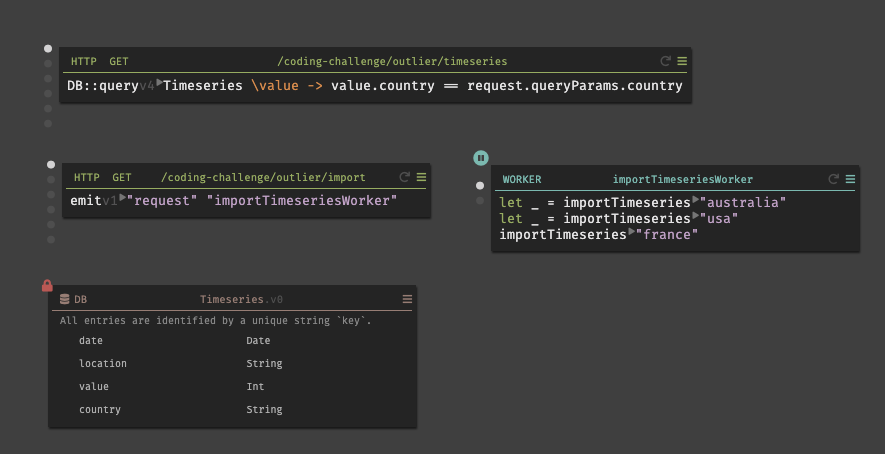
\includegraphics[width=1\linewidth]{dark.png}
  \caption{The Dark programming environment showing a simple web service comprising a database, two HTTP endpoints and a worker.\label{fig:dark}}
  \note{FROM https://medium.com/@wilk/dark-lang-an-uncommon-step-towards-the-future-of-programming-921cf7f38baf}
\end{figure}

Dark illustrates the need for the broader perspective of programming
systems. Of course, it contains a programming language, which is
inspired by OCaml and F\#. But Dark's distinguishing feature is that it
eliminates the many secondary systems needed for deployment of modern
cloud-based services. Those exist outside of a typical programming
language, yet form a major part of the complexity of the overall
development process.

With technical dimensions, we can go beyond the ``sales pitch'', look
behind the scenes, and better understand the interesting technical
aspects of Dark as a programming system.

\hypertarget{dimension-analysis-of-dark}{%
\subsubsection{Dimension analysis of
Dark}\label{dimension-analysis-of-dark}}

\paragraph{Modes of interaction and feedback loops.}

Conventional \emph{modes of interaction}
(\ref{dimension-modes-of-interaction}) include running, editing and
debugging. For modern web services, running refers to operation in a
cloud-based environment that typically comes with further kinds of
feedback (logging and monitoring). The key design decision of Dark is to
integrate all these different modes of interaction into a single one.
This tight integration allows Dark to provide a more immediate
\emph{feedback loop} (\ref{dimension-feedback-loops}) where code changes
become immediately available not just to the developer, but also to
external users. The integrated mode of interaction is reminiscent of the
image-based environment in Smalltalk; Dark advances the state of art by
using this model in a multi-user, cloud-based context.

\paragraph{Feedback loops and error response.}

The integration of development and operation also makes it possible to
use \emph{errors} occurring during operation to drive development.
Specifically, when a Dark service receives a request that is not
supported, the user can build a handler to provide a response---taking
advantage of the live data that was sent as part of the request. In
terms of our dimensions, this is a kind of \emph{error response}
(\ref{dimension-error-response}) that was pioneered by the PILOT system
for Lisp~\cite{Pilot}. Dark does this not just to respond to errors, but
also as the primary development mechanism, which we might call
\emph{Error-Driven Development.} This way, Dark users can construct
programs with respect to sample input values.

\paragraph{Conceptual structure and learnability.}

Dark programs are expressed using high-level concepts that are specific
to the domain of server-side web programming: HTTP request handlers,
databases, workers and scheduled jobs. These are designed to reduce
accidental complexity and aim for high \emph{conceptual integrity}
(\ref{dimension-conceptual-integrity-vs.-openness}). At the level of
code, Dark uses a general-purpose functional language that emphasizes
certain concepts, especially records and pipelines. The high-level
concepts contribute to \emph{learnability}
(\ref{dimension-learnability}) of the system, because they are highly
domain-specific and will already be familiar to its intended users.

\paragraph{Notational structure and uniformity.}

Dark uses a combination of graphical editor and code. The two aspects of
the notation follow the \emph{complementing notations}
(\ref{dimension-notational-structure}) pattern. The windowed interface
is used to work with the high-level concepts and code is used for
working with low-level concepts. At the high level, code is structured
in freely positionable boxes on a 2D surface. Unlike Boxer \cite{Boxer},
these boxes do not nest and the space cannot be used for other content
(say, for comments, architectural illustrations or other media). Code at
the low level is manipulated using a syntax-aware structure editor,
showing inferred types and computed live values for pure functions. It
also provides special editing support for records and pipelines,
allowing users to add fields and steps respectively.

\paragraph{Factoring of complexity and automation.}

One of the advertised goals of Dark is to remove accidental complexity.
This is achieved by collapsing the heterogeneous stack of technologies
that are typically required for development, cloud deployment,
orchestration and operation. Dark hides this via \emph{factoring of
complexity} (\ref{dimension-factoring-of-complexity}). The advanced
infrastructure is provided by the Dark platform and is hidden from the
user. The infrastructure is programmed explicitly and there is no need
for sophisticated automation (\ref{dimension-level-of-automation}). This
factoring of functionality that was previously coded manually follows a
similar pattern as the development of garbage collection in high-level
programming languages.

\paragraph{Customizability.}

The Dark platform makes a clear distinction between the platform itself
and the user application, so \emph{self-sustainability}
(\ref{dimension-self-sustainability}) is not an objective. The strict
division between the platform and user (related to its aforementioned
\emph{factoring of complexity}) means that changes to Dark require
modifying the platform source code itself, which is available under a
license that solely allows using it for the purpose of contributing.
Similarly, applications themselves are developed by modifying and adding
code, requiring destructive access to it---so \emph{additive authoring}
(\ref{dimension-addressing-and-externalizability}) is not exhibited at
either level. Thanks to the integration of execution and development,
persistent changes may be made during execution (c.f. \emph{staging of
customization}, \ref{dimension-staging-of-customization}) but this is
done through the Dark editor, which is separate from the running
service.

\hypertarget{technical-innovations-of-dark}{%
\subsubsection{Technical innovations of
Dark}\label{technical-innovations-of-dark}}

This analysis reveals a number of interesting aspects of the Dark
programming system. The first is the tight integration of different
\emph{modes of interaction} which collapses a heterogeneous stack of
technologies, makes Dark \emph{learnable}, and allows quick feedback
from deployed services. The second is the use of \emph{error response}
to guide the development of HTTP handlers. Thanks to the technical
dimensions framework, each of these can be more precisely described. It
is also possible to see how they may be supported in other programming
systems. The framework also points to possible alternatives (and perhaps
improvements) such as building a more self-sustainable system that has
similar characteristics to Dark, but allows greater flexibility in
modifying the platform from within itself.

\hypertarget{exploring-the-design-space}{%
\subsection{Exploring the design
space}\label{exploring-the-design-space}}

With a little work, technical dimensions can let us see patterns or gaps
in the design space by plotting their values on a simple scatterplot.
Here, we will look at two dimensions, \emph{notational
diversity}\footnote{This is simply the dimension we named as
  \emph{uniformity of notations}
  (\ref{dimension-uniformity-of-notations}), but flipped in the opposite
  direction.} and \emph{self-sustainability}, for the following
programming systems: Haskell, Jupyter notebooks, Boxer, HyperCard, the
Web, spreadsheets, Lisp, Smalltalk, UNIX, and COLAs.

While our choice to identify and describe dimensions as qualitative
concepts was necessary for coming up with them, \emph{some} way of
generating numbers is clearly necessary for visualizing their
relationships like this. For simplicity,\footnote{There are undoubtedly
  many ways to turn our descriptions into various measures, with
  strengths and weaknesses for different purposes, but this is beyond
  the scope of the present paper. Here, we merely wish to demonstrate
  that such a thing is possible and show what one can do with the
  results.} we adopt the following scheme. For each dimension, we
distill the main idea into several yes/no questions
(Appendix~\ref{making-dimensions-quantitative}) that capture enough of
the distinctions we observe between the systems we wish to plot. Then,
for each system, we add up the number of ``yes'' answers and obtain a
plausible score for the dimension.

\begin{figure}
  \centering
  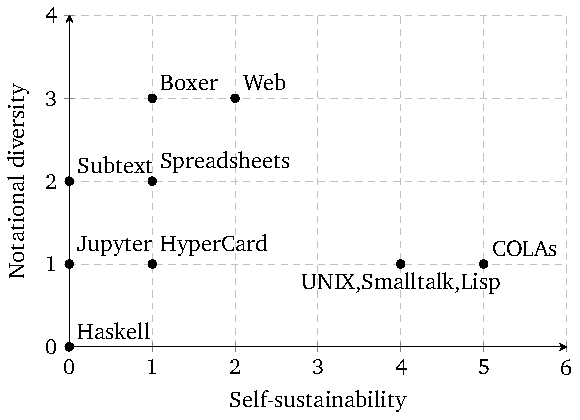
\includegraphics[width=0.6\linewidth]{plot-figure0.pdf}
  \caption{Example programming systems (or system families) measured against \emph{self-sustainability} and \emph{notational diversity}, revealing an absence of systems with a high degree of both. \label{fig:design-space-plot}}
\end{figure}

Figure~\ref{fig:design-space-plot} shows the results we obtained with
our sets of questions. It shows that the A-types span a range of
notational diversity, but only within fairly low self-sustainability.
The O-types cluster in an ``island'' at the right, sharing identical
notational diversity and near-identical self-sustainability. There is
also a conspicuous blank space at the top-right, representing an
unexplored combination of high values on both dimensions. With other
pairs of dimensions, we might take this as evidence of an oppositional
relationship, such that more of one inherently means less of the other
(perhaps looking for a single new dimension that describes this better.)
In this case, though, there is no obvious conflict between having many
notations and being able to change a system from within. Therefore, we
interpret the gap as a new opportunity to try out: combine the
self-sustainability of COLAs with the notational diversity of Boxer and
Web development. In fact, this is more or less the forthcoming
dissertation of the primary author.

\hypertarget{conclusions}{%
\section{Conclusions}\label{conclusions}}

There is a renewed interest in developing new programming systems. Such
systems go beyond the simple model of code written in a programming
language using a more or less sophisticated text editor. They combine
textual and visual notations, create programs through rich graphical
interactions, and challenge accepted assumptions about program editing,
execution and debugging. Despite the growing number of novel programming
systems, it remains difficult to evaluate the design of programming
systems and see how they improve over work done in the past. To address
the issue, we proposed a framework of ``technical dimensions'' that
captures essential characteristics of programming systems in a
qualitative but rigorous way.

The framework of technical dimensions puts the vast variety of
programming systems, past and present, on a common footing of
commensurability. This is crucial to enable the strengths of each to be
identified and, if possible, combined by designers of the next
generation of programming systems. As more and more systems are assessed
in the framework, a picture of the space of possibilities will gradually
emerge. Some regions will be conspicuously empty, indicating unrealized
possibilities that could be worth trying. In this way, a domain of
``normal science'' is created for the design of programming systems.

\acks

(To be completed for publication.)
